\documentclass[a4paper]{article} 
\addtolength{\hoffset}{-2.25cm}
\addtolength{\textwidth}{4.5cm}
\addtolength{\voffset}{-3.25cm}
\addtolength{\textheight}{5cm}
\setlength{\parskip}{0pt}
\setlength{\parindent}{0in}

%----------------------------------------------------------------------------------------
%	PACKAGES AND OTHER DOCUMENT CONFIGURATIONS
%----------------------------------------------------------------------------------------

\usepackage{blindtext} % Package to generate dummy text
\usepackage{charter} % Use the Charter font
\usepackage[utf8]{inputenc} % Use UTF-8 encoding
\usepackage{microtype} % Slightly tweak font spacing for aesthetics
\usepackage[english, ngerman]{babel} % Language hyphenation and typographical rules
\usepackage{amsthm, amsmath, amssymb} % Mathematical typesetting
\usepackage{float} % Improved interface for floating objects
\usepackage[final, colorlinks = true, 
            linkcolor = black, 
            citecolor = black]{hyperref} % For hyperlinks in the PDF
\usepackage{graphicx, multicol} % Enhanced support for graphics
\usepackage{xcolor} % Driver-independent color extensions
\usepackage{marvosym, wasysym} % More symbols
\usepackage{rotating} % Rotation tools
\usepackage{censor} % Facilities for controlling restricted text
\usepackage{listings} % Environment for non-formatted code, !uses style file!
\usepackage{pseudocode} % Environment for specifying algorithms in a natural way
 % Environment for f-structures, !uses style file!
\usepackage{booktabs} % Enhances quality of tables
\usepackage{tikz-qtree} % Easy tree drawing tool
 % Configuration for b-trees and b+-trees, !uses style file!
%\usepackage[backend=biber,style=numeric,
%            sorting=nyt]{biblatex} % Complete reimplementation of bibliographic facilities
%\addbibresource{ecl.bib}
\usepackage{csquotes} % Context sensitive quotation facilities
\usepackage[yyyymmdd]{datetime} % Uses YEAR-MONTH-DAY format for dates
\renewcommand{\dateseparator}{-} % Sets dateseparator to '-'
\usepackage{fancyhdr} % Headers and footers
\pagestyle{fancy} % All pages have headers and footers
\fancyhead{}\renewcommand{\headrulewidth}{0pt} % Blank out the default header
\fancyfoot[L]{} % Custom footer text
\fancyfoot[C]{} % Custom footer text
\fancyfoot[R]{\thepage} % Custom footer text
\newcommand{\note}[1]{\marginpar{\scriptsize \textcolor{red}{#1}}} % Enables comments in red on margin

\newcommand{\R}{\mathbb{R}}
\newcommand{\E}{\mathbb{E}}
\newcommand{\Var}{\text{Var}}
% Para poner sonrisa sobre puntos suspensivos. Uso: \overplace{n}{\dotsc}
\newcommand{\overplace}[2]{%
	\overset{\substack{#1\\\smile}}{#2}%
}

%----------------------------------------------------------------------------------------
% Generado por Rstudio al transformar desde Rmd:

\usepackage{lmodern}
\usepackage{amssymb,amsmath}
\usepackage{ifxetex,ifluatex}
\ifnum 0\ifxetex 1\fi\ifluatex 1\fi=0 % if pdftex
\usepackage[T1]{fontenc}
\usepackage[utf8]{inputenc}
\usepackage{textcomp} % provide euro and other symbols
\else % if luatex or xetex
\usepackage{unicode-math}
\defaultfontfeatures{Scale=MatchLowercase}
\defaultfontfeatures[\rmfamily]{Ligatures=TeX,Scale=1}
\fi
% Use upquote if available, for straight quotes in verbatim environments
\IfFileExists{upquote.sty}{\usepackage{upquote}}{}
\IfFileExists{microtype.sty}{% use microtype if available
	\usepackage[]{microtype}
	\UseMicrotypeSet[protrusion]{basicmath} % disable protrusion for tt fonts
}{}
\makeatletter
\@ifundefined{KOMAClassName}{% if non-KOMA class
	\IfFileExists{parskip.sty}{%
		\usepackage{parskip}
	}{% else
		\setlength{\parindent}{0pt}
		\setlength{\parskip}{6pt plus 2pt minus 1pt}}
}{% if KOMA class
	\KOMAoptions{parskip=half}}
\makeatother
\usepackage{xcolor}
\IfFileExists{xurl.sty}{\usepackage{xurl}}{} % add URL line breaks if available
\IfFileExists{bookmark.sty}{\usepackage{bookmark}}{\usepackage{hyperref}}
\hypersetup{
	pdftitle={Ejercicio 7},
	pdfauthor={José Antonio Álvarez Ocete},
	hidelinks,
	pdfcreator={LaTeX via pandoc}}
\urlstyle{same} % disable monospaced font for URLs
\usepackage[margin=1in]{geometry}
\usepackage{color}
\usepackage{fancyvrb}
\newcommand{\VerbBar}{|}
\newcommand{\VERB}{\Verb[commandchars=\\\{\}]}
\DefineVerbatimEnvironment{Highlighting}{Verbatim}{commandchars=\\\{\}}
% Add ',fontsize=\small' for more characters per line
\usepackage{framed}
\definecolor{shadecolor}{RGB}{248,248,248}
\newenvironment{Shaded}{\begin{snugshade}}{\end{snugshade}}
\newcommand{\AlertTok}[1]{\textcolor[rgb]{0.94,0.16,0.16}{#1}}
\newcommand{\AnnotationTok}[1]{\textcolor[rgb]{0.56,0.35,0.01}{\textbf{\textit{#1}}}}
\newcommand{\AttributeTok}[1]{\textcolor[rgb]{0.77,0.63,0.00}{#1}}
\newcommand{\BaseNTok}[1]{\textcolor[rgb]{0.00,0.00,0.81}{#1}}
\newcommand{\BuiltInTok}[1]{#1}
\newcommand{\CharTok}[1]{\textcolor[rgb]{0.31,0.60,0.02}{#1}}
\newcommand{\CommentTok}[1]{\textcolor[rgb]{0.56,0.35,0.01}{\textit{#1}}}
\newcommand{\CommentVarTok}[1]{\textcolor[rgb]{0.56,0.35,0.01}{\textbf{\textit{#1}}}}
\newcommand{\ConstantTok}[1]{\textcolor[rgb]{0.00,0.00,0.00}{#1}}
\newcommand{\ControlFlowTok}[1]{\textcolor[rgb]{0.13,0.29,0.53}{\textbf{#1}}}
\newcommand{\DataTypeTok}[1]{\textcolor[rgb]{0.13,0.29,0.53}{#1}}
\newcommand{\DecValTok}[1]{\textcolor[rgb]{0.00,0.00,0.81}{#1}}
\newcommand{\DocumentationTok}[1]{\textcolor[rgb]{0.56,0.35,0.01}{\textbf{\textit{#1}}}}
\newcommand{\ErrorTok}[1]{\textcolor[rgb]{0.64,0.00,0.00}{\textbf{#1}}}
\newcommand{\ExtensionTok}[1]{#1}
\newcommand{\FloatTok}[1]{\textcolor[rgb]{0.00,0.00,0.81}{#1}}
\newcommand{\FunctionTok}[1]{\textcolor[rgb]{0.00,0.00,0.00}{#1}}
\newcommand{\ImportTok}[1]{#1}
\newcommand{\InformationTok}[1]{\textcolor[rgb]{0.56,0.35,0.01}{\textbf{\textit{#1}}}}
\newcommand{\KeywordTok}[1]{\textcolor[rgb]{0.13,0.29,0.53}{\textbf{#1}}}
\newcommand{\NormalTok}[1]{#1}
\newcommand{\OperatorTok}[1]{\textcolor[rgb]{0.81,0.36,0.00}{\textbf{#1}}}
\newcommand{\OtherTok}[1]{\textcolor[rgb]{0.56,0.35,0.01}{#1}}
\newcommand{\PreprocessorTok}[1]{\textcolor[rgb]{0.56,0.35,0.01}{\textit{#1}}}
\newcommand{\RegionMarkerTok}[1]{#1}
\newcommand{\SpecialCharTok}[1]{\textcolor[rgb]{0.00,0.00,0.00}{#1}}
\newcommand{\SpecialStringTok}[1]{\textcolor[rgb]{0.31,0.60,0.02}{#1}}
\newcommand{\StringTok}[1]{\textcolor[rgb]{0.31,0.60,0.02}{#1}}
\newcommand{\VariableTok}[1]{\textcolor[rgb]{0.00,0.00,0.00}{#1}}
\newcommand{\VerbatimStringTok}[1]{\textcolor[rgb]{0.31,0.60,0.02}{#1}}
\newcommand{\WarningTok}[1]{\textcolor[rgb]{0.56,0.35,0.01}{\textbf{\textit{#1}}}}
\usepackage{graphicx,grffile}
\makeatletter
\def\maxwidth{\ifdim\Gin@nat@width>\linewidth\linewidth\else\Gin@nat@width\fi}
\def\maxheight{\ifdim\Gin@nat@height>\textheight\textheight\else\Gin@nat@height\fi}
\makeatother
% Scale images if necessary, so that they will not overflow the page
% margins by default, and it is still possible to overwrite the defaults
% using explicit options in \includegraphics[width, height, ...]{}
\setkeys{Gin}{width=\maxwidth,height=\maxheight,keepaspectratio}
% Set default figure placement to htbp
\makeatletter
\def\fps@figure{htbp}
\makeatother
\setlength{\emergencystretch}{3em} % prevent overfull lines
\providecommand{\tightlist}{%
	\setlength{\itemsep}{0pt}\setlength{\parskip}{0pt}}
\setcounter{secnumdepth}{-\maxdimen} % remove section numbering


\usepackage{mathtools}
\usepackage{amsmath}
\usepackage[shortlabels]{enumitem}
\DeclarePairedDelimiter\abs{\lvert}{\rvert}%
\usepackage{cancel}

\begin{document}

%-------------------------------
%	TITLE SECTION
%-------------------------------

\fancyhead[C]{}
\hrule \medskip % Upper rule
\begin{minipage}{0.295\textwidth} 
\raggedright
\footnotesize
José Antonio Álvarez Ocete \hfill\\   
77553417Q \hfill\\
joseantonio.alvarezo@estudiante.uam.es
\end{minipage}
\begin{minipage}{0.4\textwidth} 
\centering 
\large 
Ejercicios\\ 
\normalsize 
Métodos Avanzados en Estadística\\ 
\end{minipage}
\begin{minipage}{0.295\textwidth} 
\raggedleft
\today\hfill\\
\end{minipage}
\medskip\hrule 
\bigskip
	
%-------------------------------
%	CONTENTS
%-------------------------------

\section*{Ejercicio 2.}

\textbf{Enunciado.} Sea $X_1, \ldots, X_n$ una muestra de $n$ observaciones \emph{iid} de una distribución $F$ con esperanza $\mu$ y varianza $\sigma^2$, y sea $X_1^*, \ldots, X_n^*$ una muestra de $n$ observaciones de la distribución empírica de la muestra original $F_n$. Calcula las siguientes cantidades: \\

\begin{enumerate}[a)]
	\item $\E_{F_n}(\bar X_n^*) := \E(\bar X_n^* | X_1, \ldots, X_n)$
	
	Esta esperanza nos supone un cálculo directo utilizando la linealidad de la esperanza:
	
	\[
		\E_{F_n}(\bar X_n^*) = \E_{F_n} \bigg( \frac{1}{n} \sum_{i=1}^n X_i^* \bigg) = \frac{1}{n} \sum_{i=1}^n \E_{F_n}(X_i^*) \stackrel{\text{iid}}{=} \frac{1}{n} \cdot n \ \E_{F_n}(X_1^*) = \bar x
	\]
	
	\item $\E_{F}(\bar X_n^*)$
	
	Por un proceso análogo al anterior podemos obtener que:
	
	\[
		\E_{F}(\bar X_n^*) = \E_{F} \bigg( \frac{1}{n} \sum_{i=1}^n X_i^* \bigg) = \frac{1}{n} \sum_{i=1}^n \E_{F}(X_i^*) \stackrel{\text{iid}}{=} \frac{1}{n} \cdot n \ \E_{F}(X_1^*) = \E_{F}(X_1^*)
	\]
	
	Sin embargo, $\E_{F}(X_1^*)$ no se puede calcular directamente pues depende de la muestra tomada $X_1, \ldots, X_n$. Podemos utilizar la \textbf{ley de la esperanza iterada}$\E[Y] = \E(\E(Y|X))$ y el valor calculado en el apartado anterior:
		
	\[
		\E_{F}(X_1^*) = \E_{F}(\E(X_1^* | X_1, \ldots, X_n)) = \E_{F}(\E_{F_n}(X_1^*)) = \E_{F}(\bar x) = \mu
	\]
	
	\item $\Var_{F_n}(\bar X_n^*) := Var(\bar X_n^* | X_1, \ldots, X_n)$
	
	Expresaremos esta varianza en función de la varianza muestra insesgada:
	
	\[
		s^2 = \frac{1}{n-1} \bigg( \sum_i x_i^2 - n \bar x^2 \bigg) = \frac{n}{n-1} \bigg( \frac{1}{n}\sum_i x_i^2 - \bar x^2 \bigg)
	\]
	
	Al ser insesgada, sabemos que $\E[s^2] = \sigma^2$. Esto nos será útil en el último apartado. Procedamos con el cálculo de la varianza:
		
	\[
		\begin{split}
			\Var_{F_n}(\bar X_n^*) & \stackrel{\text{iid}}{=} \frac{1}{n^2} \sum_{i=1}^n \Var_{F_n}(X_i^*) \\
			& \stackrel{\text{iid}}{=} \frac{1}{n^2} \cdot n \ \Var_{F_n}(X_1^*) \\
			& = \frac{1}{n} \bigg( \E_{F_n}( {X_1^*}^2 ) - \E_{F_n}( X_1^* )^2 \bigg) \\
			& = \frac{1}{n} \bigg( \frac{1}{n} \sum_{i=1}^n X_i^2 - \bar x^2 \bigg) \\
			& = \frac{n-1}{n^2} \underbrace{\frac{n}{n-1} \bigg( \frac{1}{n} \sum_{i=1}^n X_i^2 - \bar x^2 \bigg)}_{s^2} \\
			& = \frac{n-1}{n^2} s^2 \\
		\end{split}
	\]
	
	\item $Var_{F}(\bar X_n^*)$
	
	Para este último apartado haremos uso de la \textbf{ley de la varianza total}:
	
	\[
		\Var(Y) = \E(\Var(Y|X)) + \Var(\E(Y|X))
	\]
	
	Procedemos con el cálculo de la varianza:
	
	\[
		\begin{split}
			\Var_{F}(\bar X_n^*) & = \E_{F}( \underbrace{\Var_{F_n}(\bar X^*_n)}_{\frac{n-1}{n^2} s^2} ) + \Var_{F}( \underbrace{\E_{F_n}(\bar X^*_n)}_{\bar x} )\\
			& = \frac{n-1}{n^2} \E_{F}(s^2) + \Var_{F}( \bar x ) \\
			& \stackrel{\text{iid}}{=} \frac{n-1}{n^2} \sigma^2 + \frac{1}{n} \Var_{F}(X_1)  \\
			& = \frac{n-1}{n^2} \sigma^2 + \frac{1}{n} \sigma^2 \\
			& = \frac{2n-1}{n^2} \sigma^2 \\
		\end{split}
	\]
	
\end{enumerate}

\section*{Ejercicio 7.}

Importamos los paquetes necesarios:

\begin{Shaded}
	\begin{Highlighting}[]
		\KeywordTok{library}\NormalTok{(tidyverse)}
		\KeywordTok{library}\NormalTok{(gapminder)}
		\KeywordTok{library}\NormalTok{(comprehenr)}
		\KeywordTok{library}\NormalTok{(ggplot2)}
		\KeywordTok{library}\NormalTok{(dplyr)}
		\KeywordTok{theme_set}\NormalTok{(}\KeywordTok{theme_bw}\NormalTok{())}
	\end{Highlighting}
\end{Shaded}

Implementamos una función que calcula el coeficiente de asimetría
muestral de una muestra dada. Utilizaremos el estimador natural:
sustituir la esperanza por el promedio de los valores, la media por la
media muestral y la varianza por la varianza muestral, siendo
conscientes de que esta varianza muestra es \(s^2\) y no \(\sigma^2\).

\begin{Shaded}
	\begin{Highlighting}[]
		\NormalTok{asymmetry_coefficient <-}\StringTok{ }\ControlFlowTok{function}\NormalTok{(muestra) \{}
		\NormalTok{  mean <-}\StringTok{ }\KeywordTok{mean}\NormalTok{(muestra)}
		\NormalTok{  sigma <-}\StringTok{ }\KeywordTok{sd}\NormalTok{(muestra)}
		\KeywordTok{mean}\NormalTok{((muestra }\OperatorTok{-}\StringTok{ }\NormalTok{mean)}\OperatorTok{^}\DecValTok{3} \OperatorTok{/}\StringTok{ }\NormalTok{sigma)}
		\NormalTok{\}}
	\end{Highlighting}
\end{Shaded}

Implementamos una función que pinta los intervalos alrededor del valor
real \(\theta\), sirviéndonos del código proporcionado en las
diapositivas.

\begin{Shaded}
	\begin{Highlighting}[]
		\NormalTok{plot_intervals <-}\StringTok{ }\ControlFlowTok{function}\NormalTok{(intervals, hits, theta, method_name, distribution_name) \{}
		\NormalTok{  m <-}\StringTok{ }\KeywordTok{nrow}\NormalTok{(intervals)}
		\NormalTok{  df <-}\StringTok{ }\KeywordTok{data.frame}\NormalTok{(ic_min <-}\StringTok{ }\NormalTok{intervals[,}\DecValTok{1}\NormalTok{],}
		\NormalTok{                   ic_max <-}\StringTok{ }\NormalTok{intervals[,}\DecValTok{2}\NormalTok{],}
		\DataTypeTok{ind =} \DecValTok{1}\OperatorTok{:}\NormalTok{m,}
		\DataTypeTok{hits =}\NormalTok{ hits)}
		
		\NormalTok{  gg <-}\StringTok{ }\KeywordTok{ggplot}\NormalTok{(df) }\OperatorTok{+}
		\StringTok{    }\KeywordTok{geom_linerange}\NormalTok{(}\KeywordTok{aes}\NormalTok{(}\DataTypeTok{xmin=}\NormalTok{ic_min, }\DataTypeTok{xmax=}\NormalTok{ic_max, }\DataTypeTok{y=}\NormalTok{ind, }\DataTypeTok{col=}\NormalTok{hits)) }\OperatorTok{+}
		\StringTok{    }\KeywordTok{scale_color_hue}\NormalTok{(}\DataTypeTok{labels =} \KeywordTok{c}\NormalTok{(}\StringTok{"NO"}\NormalTok{, }\StringTok{"SÍ"}\NormalTok{)) }\OperatorTok{+}
		\StringTok{    }\KeywordTok{geom_vline}\NormalTok{(}\KeywordTok{aes}\NormalTok{(}\DataTypeTok{xintercept =}\NormalTok{ theta), }\DataTypeTok{linetype =} \DecValTok{2}\NormalTok{) }\OperatorTok{+}
		\StringTok{    }\KeywordTok{theme_bw}\NormalTok{() }\OperatorTok{+}
		\StringTok{    }\KeywordTok{labs}\NormalTok{(}\DataTypeTok{y =} \StringTok{'Muestras'}\NormalTok{, }\DataTypeTok{x =} \StringTok{'Intervalos (nivel 0.95)'}\NormalTok{,}
		\DataTypeTok{title =} \KeywordTok{paste}\NormalTok{(}\StringTok{'IC -'}\NormalTok{, method_name, }\StringTok{'para'}\NormalTok{, distribution_name, }\DataTypeTok{sep=}\StringTok{' '}\NormalTok{))}
		\KeywordTok{print}\NormalTok{(gg)}
		\NormalTok{\}}
	\end{Highlighting}
\end{Shaded}

Implementamos dos funciones auxiliares adicionales. La primera muestra
una distribución (normal o exponencial) \texttt{n} veces. La segunda
calcula el intervalo de confianza del coeficiente de asimetría
utilizando el método proporcionado por parámetro.

\begin{Shaded}
	\begin{Highlighting}[]
		\NormalTok{sample_dist <-}\StringTok{ }\ControlFlowTok{function}\NormalTok{(distribution, n) \{}
		\ControlFlowTok{if}\NormalTok{ (distribution }\OperatorTok{==}\StringTok{ 'normal'}\NormalTok{) \{}
		\KeywordTok{rnorm}\NormalTok{(n, }\DecValTok{0}\NormalTok{, }\DecValTok{1}\NormalTok{)}
		\NormalTok{  \} }\ControlFlowTok{else} \ControlFlowTok{if}\NormalTok{ (distribution }\OperatorTok{==}\StringTok{ 'exponential'}\NormalTok{) \{}
		\KeywordTok{rexp}\NormalTok{(n, }\DecValTok{1}\NormalTok{)}
		\NormalTok{  \} }\ControlFlowTok{else}\NormalTok{ \{}
		\KeywordTok{print}\NormalTok{(}\StringTok{'Distribution not supported'}\NormalTok{)}
		\NormalTok{  \}}
		\NormalTok{\}}
		
		\NormalTok{compute_interval <-}\StringTok{ }\ControlFlowTok{function}\NormalTok{(method, gammas_bootstrap, gamma_original, alfa) \{}
		\ControlFlowTok{if}\NormalTok{ (method }\OperatorTok{==}\StringTok{ 'Método híbrido'}\NormalTok{) \{}
		\CommentTok{# Metodo hibrido}
		\NormalTok{    n =}\StringTok{ }\KeywordTok{length}\NormalTok{(gammas_bootstrap)}
		\NormalTok{    T_bootstrap <-}\StringTok{ }\KeywordTok{sqrt}\NormalTok{(n) }\OperatorTok{*}\StringTok{ }\NormalTok{(gammas_bootstrap }\OperatorTok{-}\StringTok{ }\NormalTok{gamma_original)}
		\NormalTok{    ic_min <-}\StringTok{ }\NormalTok{gamma_original }\OperatorTok{-}\StringTok{  }\KeywordTok{quantile}\NormalTok{(T_bootstrap, }\DecValTok{1}\OperatorTok{-}\NormalTok{alfa}\OperatorTok{/}\DecValTok{2}\NormalTok{)}\OperatorTok{/}\KeywordTok{sqrt}\NormalTok{(n)}
		\NormalTok{    ic_max  <-}\StringTok{ }\NormalTok{gamma_original }\OperatorTok{-}\StringTok{  }\KeywordTok{quantile}\NormalTok{(T_bootstrap, alfa}\OperatorTok{/}\DecValTok{2}\NormalTok{)}\OperatorTok{/}\KeywordTok{sqrt}\NormalTok{(n)}
		\KeywordTok{c}\NormalTok{(ic_min, ic_max)}
		\NormalTok{  \} }\ControlFlowTok{else} \ControlFlowTok{if}\NormalTok{ (method }\OperatorTok{==}\StringTok{ 'Método normal'}\NormalTok{) \{}
		\CommentTok{# Metodo normal}
		\NormalTok{    et_boostrap <-}\StringTok{ }\KeywordTok{sd}\NormalTok{(gammas_bootstrap)}
		\NormalTok{    ic_min <-}\StringTok{ }\NormalTok{gamma_original }\OperatorTok{+}\StringTok{ }\KeywordTok{qnorm}\NormalTok{(alfa}\OperatorTok{/}\DecValTok{2}\NormalTok{, }\DecValTok{0}\NormalTok{, }\DecValTok{1}\NormalTok{)}\OperatorTok{*}\NormalTok{et_boostrap}
		\NormalTok{    ic_max  <-}\StringTok{ }\NormalTok{gamma_original }\OperatorTok{-}\StringTok{ }\KeywordTok{qnorm}\NormalTok{(alfa}\OperatorTok{/}\DecValTok{2}\NormalTok{, }\DecValTok{0}\NormalTok{, }\DecValTok{1}\NormalTok{)}\OperatorTok{*}\NormalTok{et_boostrap}
		\KeywordTok{c}\NormalTok{(ic_min, ic_max)}
		\NormalTok{  \} }\ControlFlowTok{else} \ControlFlowTok{if}\NormalTok{ (method }\OperatorTok{==}\StringTok{ 'Método percentil'}\NormalTok{) \{}
		\CommentTok{# Metodo percentil}
		\NormalTok{    ic_min <-}\StringTok{ }\KeywordTok{quantile}\NormalTok{(gammas_bootstrap, alfa}\OperatorTok{/}\DecValTok{2}\NormalTok{)}
		\NormalTok{    ic_max  <-}\StringTok{ }\KeywordTok{quantile}\NormalTok{(gammas_bootstrap, }\DecValTok{1}\OperatorTok{-}\NormalTok{alfa}\OperatorTok{/}\DecValTok{2}\NormalTok{)}
		\KeywordTok{c}\NormalTok{(ic_min, ic_max)}
		\NormalTok{  \} }\ControlFlowTok{else}\NormalTok{ \{}
		\KeywordTok{print}\NormalTok{(}\StringTok{'Method not supported'}\NormalTok{)}
		\NormalTok{  \}}
		\NormalTok{\}}
	\end{Highlighting}
\end{Shaded}

Utilizando las funciones anteriores implementamos una función final que,
dada una distibución y un método, calcula \texttt{n=100} muestras
originales, remuestrea \texttt{R=1000} veces y calcula el intervalor de
confianza para el coeficiente de asimetría. Repetimos este proceso
\texttt{m=1000} veces y dibujamos los distintos intervalos de confianza.
Adicionalmente se mostrará la precisión del método.

\begin{Shaded}
	\begin{Highlighting}[]
		\NormalTok{exercise_}\DecValTok{2}\NormalTok{ <-}\StringTok{ }\ControlFlowTok{function}\NormalTok{ (distribution, method) \{}
		\NormalTok{  R <-}\StringTok{ }\DecValTok{1000}
		\NormalTok{  n <-}\StringTok{ }\DecValTok{100}
		\NormalTok{  m <-}\StringTok{ }\DecValTok{1000}
		
		\NormalTok{  alfa <-}\StringTok{ }\FloatTok{0.05}
		\NormalTok{  theta =}\StringTok{ }\ControlFlowTok{if}\NormalTok{ (distribution }\OperatorTok{==}\StringTok{ 'normal'}\NormalTok{) }\DecValTok{0} \ControlFlowTok{else} \DecValTok{2}
		
		\NormalTok{  intervalos <-}\StringTok{ }\OtherTok{NULL}
		\NormalTok{  aciertos <-}\StringTok{ }\OtherTok{NULL}
		
		\ControlFlowTok{for}\NormalTok{ (i }\ControlFlowTok{in} \DecValTok{1}\OperatorTok{:}\NormalTok{m) \{}
		\CommentTok{# Usar la distribución para muestrear}
		\NormalTok{    muestra_original <-}\StringTok{ }\KeywordTok{sample_dist}\NormalTok{(distribution, n)}
		\NormalTok{    gamma_original <-}\StringTok{ }\KeywordTok{asymmetry_coefficient}\NormalTok{(muestra_original)}
		
		\CommentTok{# Muestreo boostrap y computar los estimadores boostrap}
		\NormalTok{    muestras_bootstrap <-}\StringTok{ }\KeywordTok{sample}\NormalTok{(muestra_original, n}\OperatorTok{*}\NormalTok{R, }\DataTypeTok{rep =} \OtherTok{TRUE}\NormalTok{)}
		\NormalTok{    muestras_bootstrap <-}\StringTok{ }\KeywordTok{matrix}\NormalTok{(muestras_bootstrap, }\DataTypeTok{nrow =}\NormalTok{ n)}
		\NormalTok{    gammas_bootstrap <-}\StringTok{ }\KeywordTok{apply}\NormalTok{(muestras_bootstrap, }\DecValTok{2}\NormalTok{, asymmetry_coefficient)}
		
		\CommentTok{# Computar el intervalo y el acierto}
		\NormalTok{    interv <-}\StringTok{ }\KeywordTok{compute_interval}\NormalTok{(method, gammas_bootstrap, gamma_original, alfa)}
		\NormalTok{    intervalos <-}\StringTok{ }\KeywordTok{rbind}\NormalTok{(intervalos, interv)}
		\NormalTok{    aciertos <-}\StringTok{ }\KeywordTok{c}\NormalTok{(aciertos, interv[}\DecValTok{1}\NormalTok{] }\OperatorTok{<}\StringTok{ }\NormalTok{theta }\OperatorTok{&}\StringTok{ }\NormalTok{interv[}\DecValTok{2}\NormalTok{] }\OperatorTok{>}\StringTok{ }\NormalTok{theta)}
		\NormalTok{  \}}
		
		\CommentTok{# Cálculo del accuracy}
		\NormalTok{  acc =}\StringTok{ }\DecValTok{100} \OperatorTok{*}\StringTok{ }\KeywordTok{length}\NormalTok{(aciertos[aciertos }\OperatorTok\StringTok{ }\OtherTok{TRUE}\NormalTok{]) }\OperatorTok{/}\StringTok{ }\NormalTok{m}
			\KeywordTok{print}\NormalTok{(}\KeywordTok{paste}\NormalTok{(method, }\StringTok{' - accuracy: '}\NormalTok{, acc, }\StringTok{'%'}\NormalTok{, }\DataTypeTok{separator=}\StringTok{''}\NormalTok{))}
				
				\CommentTok{# Gráfico}
				\NormalTok{  distribution_name =}\StringTok{ }\ControlFlowTok{if}\NormalTok{ (distribution }\OperatorTok{==}\StringTok{ 'normal'}\NormalTok{) }\StringTok{'N(0,1))'} \ControlFlowTok{else} \StringTok{'exp(1)'}
				\KeywordTok{plot_intervals}\NormalTok{(intervalos, aciertos, theta,}
				\NormalTok{                 method, distribution_name)}
				\NormalTok{\}}
			\end{Highlighting}
		\end{Shaded}
		
		Utilizamos la función anterior para mostrar los distintos intervalos de
		confianza para la normal, así como su precisión.
		
		\begin{Shaded}
			\begin{Highlighting}[]
				\KeywordTok{set.seed}\NormalTok{(}\DecValTok{123}\NormalTok{)}
				
				\NormalTok{methods <-}\StringTok{ }\KeywordTok{c}\NormalTok{(}\StringTok{'Método híbrido'}\NormalTok{, }\StringTok{'Método normal'}\NormalTok{, }\StringTok{'Método percentil'}\NormalTok{)}
				\ControlFlowTok{for}\NormalTok{ (method }\ControlFlowTok{in}\NormalTok{ methods) \{}
				\KeywordTok{exercise_2}\NormalTok{(}\StringTok{'normal'}\NormalTok{, method)}
				\NormalTok{\}}
			\end{Highlighting}
		\end{Shaded}
		
		\begin{verbatim}
			## [1] "Método híbrido  - accuracy:  95.2 % "
		\end{verbatim}
		
		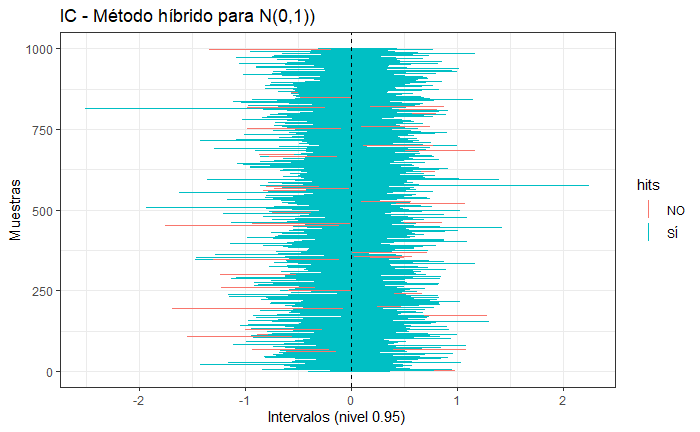
\includegraphics{figures/norm1.png}
		
		\begin{verbatim}
			## [1] "Método normal  - accuracy:  94.8 % "
		\end{verbatim}
		
		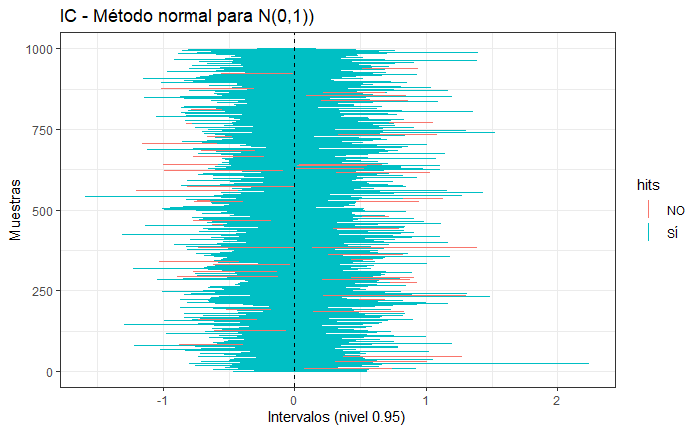
\includegraphics{figures/norm2.png}
		
		\begin{verbatim}
			## [1] "Método percentil  - accuracy:  94.6 % "
		\end{verbatim}
		
		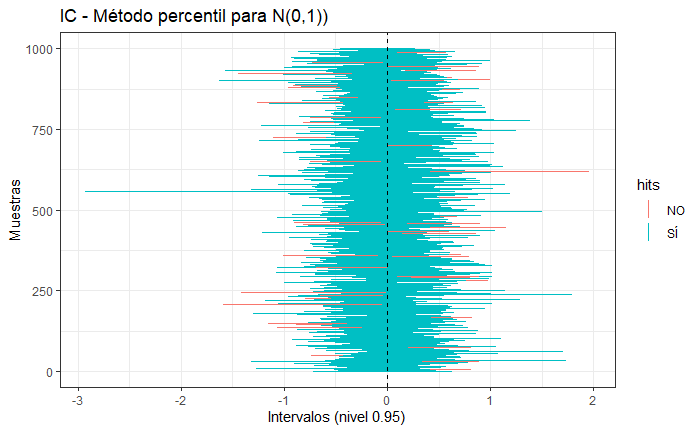
\includegraphics{1figures/norm3.png}
		
		Obtenemos así precisiones cercanas al 95\%. Este resultado era de
		esperar pues tomamos \texttt{alfa=0.05}. Repetimos el experimento para
		la distribución exponencial con parámetro \(\lambda=1\).
		
		\begin{Shaded}
			\begin{Highlighting}[]
				\NormalTok{methods <-}\StringTok{ }\KeywordTok{c}\NormalTok{(}\StringTok{'Método híbrido'}\NormalTok{, }\StringTok{'Método normal'}\NormalTok{, }\StringTok{'Método percentil'}\NormalTok{)}
				\ControlFlowTok{for}\NormalTok{ (method }\ControlFlowTok{in}\NormalTok{ methods) \{}
				\KeywordTok{exercise_2}\NormalTok{(}\StringTok{'exponential'}\NormalTok{, method)}
				\NormalTok{\}}
			\end{Highlighting}
		\end{Shaded}
		
		\begin{verbatim}
			## [1] "Método híbrido  - accuracy:  65.3 % "
		\end{verbatim}
		
		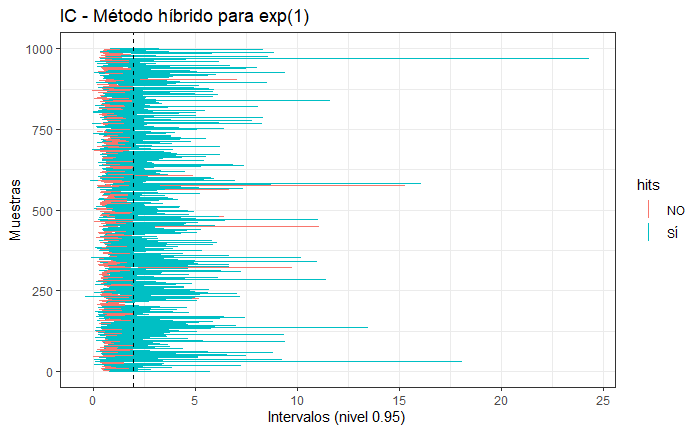
\includegraphics{figures/exp1.png}
		
		\begin{verbatim}
			## [1] "Método normal  - accuracy:  68 % "
		\end{verbatim}
		
		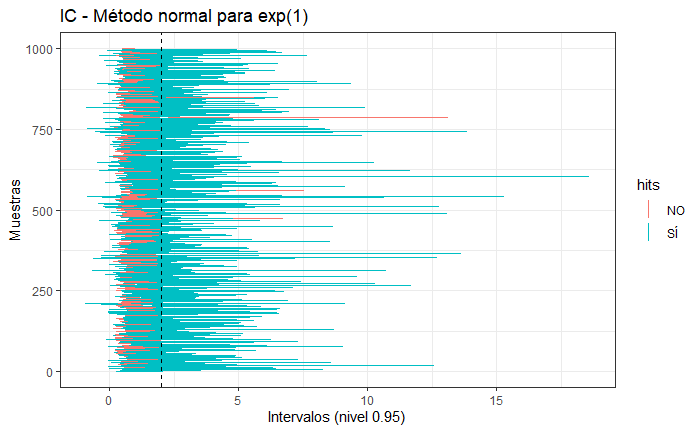
\includegraphics{figures/exp2.png}
		
		\begin{verbatim}
			## [1] "Método percentil  - accuracy:  63.6 % "
		\end{verbatim}
		
		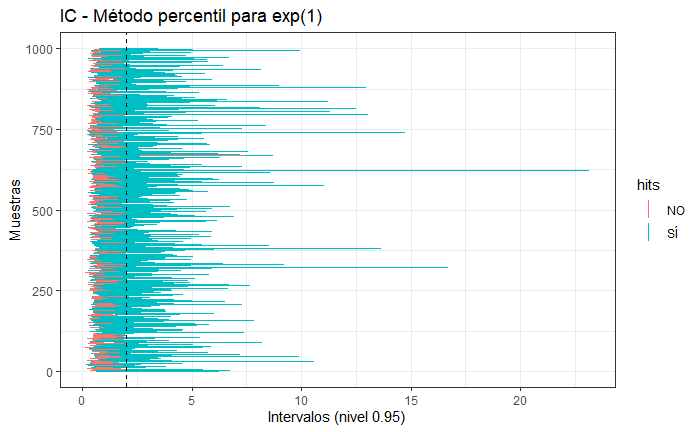
\includegraphics{figures/exp3.png}
		
		En este caso, el coeficiente de asimetría real es 2. Sin embargo, vemos
		como obtenemos una precisión mucho menor: entorno al 65\% en los
		diferentes métodos. Esto puede deberse a que el coeficiente de asimetría
		no se estime correctamente utilizando boostrap.

\end{document}
